%%
\documentclass[%
]{ittmm}

\graphicspath{ {./assets/} }

\usepackage{hyperref}
\usepackage{tabularx}
\usepackage{polyglossia}
\setdefaultlanguage[spelling=modern]{russian}
\setotherlanguages{english}

%%% One can fix some overfulls
\sloppy

%% Minted listings support
%% Need pygment <http://pygments.org/> <http://pypi.python.org/pypi/Pygments>
\usepackage{minted}
%% auto break lines
\setminted{breaklines=true}

\addbibresource{main.bib}

%% end of the preamble, start of the body of the document source.
\begin{document}

\selectlanguage{russian}

%%
%% Rights management information.
%% CC-BY is default license.
\copyrightyear{2025}
\copyrightclause{Copyright for this paper by its authors.
  Use permitted under Creative Commons License Attribution 4.0
  International (CC BY 4.0).}

%%
%% This command is for the conference information
\conference{Information and Telecommunication Technologies and Mathematical Modeling of High-Tech Systems 2025 (ITTMM 2025), Moscow, April 07--11, 2025}

%%
%% The "title" command
\title{Разрешение конфликтов и кооперативное планирование в мультиагентных системах}
\title[mode=trans]{Conflict Solving and Cooperated Planning in Multi-agent Systems}

% \tnotemark[1]
% \tnotetext[1]{You can use this document as the template for preparing your publication. We recommend using the latest version of the ittmm style.}

%%
%% The "author" command and its associated commands are used to define
%% the authors and their affiliations.
\author[1]{Григорий В. Матюхин}[%
trans={Grigorii V. Matiukhin},
email=contact@gmatiukhin.site,
orcid=0000-0001-8727-5119,
url=https://gmatiukhin.site,
]
\cormark[1]

\author[1]{Андрей Н. Виноградов}[%
trans={Andrei N. Vinogradov},
email=vinogradov-an@rudn.ru,
orcid=0000-0002-3349-8859,
]
\address[1]{Российский университет дружбы народов, ул. Миклухо-Маклая, д. 6, Москва, 117198, Российская Федерация}

%%% Footnotes
\cortext[1]{Автор, отвечающий за публикацию.}

%%
%% The abstract is a short summary of the work to be presented in the
%% article.
\begin{abstract}
  В данной работе рассматривается задача разрешения конфликтов и кооперативного
  планирования в мультиагентных системах, которые находят широкое применение
  в различных областях, включая робототехнику, логистику, киберфизические системы
  и распределенные вычисления. Проведен систематический обзор существующих
  методологий, направленных на координацию действий агентов в динамических
  и неопределенных средах. Особое внимание уделяется переговорам,
  аргументационно-ориентированным методам и децентрализованным механизмам
  управления, обеспечивающим согласованность решений агентов при наличии
  конфликтующих целей.

  Анализируются ключевые подходы к моделированию мультиагентных систем,
  включая задачи удовлетворения ограничений, иерархические сетевые структуры
  и временные модели. Рассматриваются стратегии разрешения конфликтов, такие как
  ослабление ограничений, методы согласования и алгоритмы распределенного консенсуса.
  Также изучаются механизмы кооперативного планирования, ориентированные
  на иерархическую декомпозицию задач, распределенное управление и динамическую
  адаптацию стратегий агентов. Оценивается эффективность данных методов с точки зрения
  вычислительных затрат, масштабируемости и адаптивности к изменяющимся условиям среды.

  Выявлены основные ограничения существующих решений, включая недостаточную
  стандартизацию методов оценки, сложности в обеспечении надежности взаимодействия
  агентов и нехватку исследований, ориентированных на реальные сценарии применения.
  В заключение предложены рекомендации по совершенствованию стратегий
  кооперативного взаимодействия и управления конфликтами, а также перспективные
  направления дальнейших исследований, направленные на повышение адаптивности,
  устойчивости и вычислительной эффективности мультиагентных систем.
\end{abstract}

%%
%% Keywords. The author(s) should pick words that accurately describe
%% the work being presented. Separate the keywords with commas.
\begin{keywords}
  Разрешение конфликтов \sep
  Кооперативное планирование \sep
  Мультиагентные системы \sep
  Систематический обзор
\end{keywords}

%% This command processes the author and affiliation and title
%% information and builds the first part of the formatted document.
\maketitle

\section{Введение}
\label{sec:intro}

Мультиагентные системы (MAS, \textit{Multi-Agent System}) играют центральную роль в искусственном интеллекте,
обеспечивая децентрализованное принятие решений в таких областях, как автономные
транспортные средства, интеллектуальные энергосистемы и робототехника~\cite{Torre_o_2017}.
Их масштабируемость, адаптивность и отказоустойчивость делают их незаменимыми
для сложных, динамических сред, требующих кооперации и разрешения конфликтов.

Несмотря на достижения, остаются проблемы, связанные с эффективной координацией
и разрешением конфликтов~\cite{galesloot2024factoredonlineplanningmanyagent}
\cite{zhang2014formalanalysisrequiredcooperation}. Такие методы, как задачи удовлетворения
ограничений (CSP, \textit{Constraint Satisfaction Problem})~\cite{KOMENDA201476} и модели, основанные на переговорах
\cite{GROSZ1996269,RABELO1994303}, демонстрируют потенциал, но часто сталкиваются
с проблемами масштабируемости в реальных условиях. Кроме того, отсутствие единых
оценочных метрик затрудняет сравнительный анализ.

В этом обзоре систематически анализируются методологии и исследовательские пробелы
с использованием PRISMA-ScR~\cite{prisma-src}, с акцентом на моделирование предметной
области, разрешение конфликтов и механизмы кооперации. Цель — предоставить основу
для будущих разработок MAS, способствующих их более широкому применению в реальных
сценариях.

Ключевые цели исследования:

\begin{enumerate}
  \item Определение распространенных подходов к моделированию MAS.
  \item Анализ стратегий разрешения конфликтов.
  \item Исследование механизмов кооперации.
  \item Оценка эффективности существующих методологий.
\end{enumerate}

\section{Методы} 
\label{sec:methods}

\subsection{Протокол и регистрация}

Настоящий обзор следует структуре PRISMA-ScR~\cite{prisma-src},
обеспечивая систематичность и прозрачность изложения.
Перед сбором данных были определены исследовательские цели,
критерии включения и стратегии поиска.
Протокол не был зарегистрирован в PROSPERO,
так как скопинговые обзоры не входят в его сферу.\footnote{С протоколом можно ознакомится по ссылке 
\url{https://gmatiukhin.site/articles/MAS-Conflict-Solving-Review/}}

\subsection{Критерии отбора}

Обзор основан на структуре «Популяция, Концепция, Контекст» (PCC, \textit{Population, Concept, Context})~\cite{afc61c6cf471416489e36a4bc382d3b9}.
В него включены исследования, посвященные методам кооперации в системах с несколькими автономными агентами.
Под <<автономным агентом>> понимается интеллектуальный объект,
способный воспринимать окружающую среду,
принимать решения и действовать самостоятельно в рамках вычислительных и коммуникационных ограничений.
Это определение не ограничивается только роботами или беспилотными транспортными средствами.

Обзор включает как качественные, 
так и количественные эмпирические исследования,
исключая комментарии, аналитические заметки и тезисы конференций.

\begin{table}
  \centering
  \caption{Критерии включения/исключения}
  \label{tab:criteria}
  \begin{tabularx}{\textwidth}{|X|X|X|X|}
    \hline
    Критерий & Включение & Исключение & Обоснование\\
    \hline
    \hline
 Популяция        & Системы с несколькими автономными агентами, работающими как в реальных (роевые роботы, системы доставки), так и в виртуальных или симулированных средах. & Системы с одним агентом.                                                              & В обзоре рассматриваются кооперация и разрешение конфликтов, что неактуально для систем с одним агентом.                  \\
    \hline
 Концепция        & Алгоритмы, обеспечивающие кооперацию между автономными агентами в MAS.                                                                                   & Алгоритмы, ориентированные только на одиночные агенты.                                & Обзор сосредоточен на алгоритмах, способствующих кооперации в MAS.                                                        \\
    \hline
 Контекст         & Исследования, посвященные разработке алгоритмов кооперативного планирования и разрешения конфликтов в MAS с элементами искусственного интеллекта.        & Исследования, касающиеся разрешения конфликтов вне области искусственного интеллекта. & Обзор ориентирован исключительно на алгоритмы в области искусственного интеллекта, остальные области не рассматриваются.  \\
    \hline
 Язык             & Английский, русский, немецкий.                                                                                                                           & Другие языки.                                                                         & Рецензенты владеют только английским, русским и немецким языками и не имеют ресурсов для перевода статей с других языков. \\
    \hline
 Типы источников  & Рецензируемые научные статьи, эмпирические исследования.                                                                                                 & Нерецензируемые статьи, комментарии, письма в редакцию.                               & Использование рецензируемых источников гарантирует надежность и научную обоснованность представленных данных.             \\
    \hline
 Географический   & Любые страны.                                                                                                                                            & Нет исключений.                                                                       & Исследование кооперации и разрешения конфликтов в MAS не зависит от страны происхождения.                                 \\
    \hline
 Временной период & Любой.                                                                                                                                                   & Нет исключений.                                                                       & Область исследования достаточно узкая, поэтому решено включить все доступные научные работы.                              \\
    \hline
  \end{tabularx}
\end{table}

\subsection{Источники информации}

Поиск литературы проводился преимущественно в ScienceDirect,
выбранном из-за его обширного репозитория рецензируемых статей
по разрешению конфликтов и кооперации в MAS.

Дополнительно проводился поиск по цитированиям для выявления
важных исследований, которые могли быть пропущены. Списки литературы
включенных исследований были вручную проверены на наличие других
потенциально релевантных источников.

\subsection{Стратегия поиска}

Стратегия поиска была разработана для систематического выявления научных статей по кооперации в MAS.
Первичный поиск помог определить соответствующую терминологию и исследовательские темы,
что позволило уточнить ключевые слова для поиска.
Были применены расширенные методики, включая булевы операторы и усечение слов,
для охвата лексических вариаций и расширения обзора литературы.
Итеративный процесс адаптировался к возникающим инсайтам,
а ручной анализ списков литературы дополнял электронные поиски,
помогая выявить ключевые исследования.
Такой подход обеспечил комплексное изучение предметных аспектов в области MAS.

Использованные поисковые запросы:

\begin{itemize}
  \item \texttt{multi-agent systems AND conflict solving}
  \item \texttt{cooperated planning AND conflict solving}
  \item \texttt{multi-agent systems AND cooperated planning}
  \item \texttt{multi-agent systems AND (cooperated planning OR conflict solving)}
\end{itemize}

\subsection{Выбор источников данных}

Заголовки и аннотации найденных статей проверялись одним рецензентом.
Статьи, в отношении которых возникали сомнения, передавались
на полное текстовое рассмотрение. Статьи, соответствующие
критериям включения (таблица~\ref{tab:criteria}), анализировались в полном объеме
одним рецензентом. Итоговые результаты поиска, включая количество
отобранных и отклоненных статей на каждом этапе, были представлены
в виде диаграммы потока PRISMA (рис.~\ref{fig:PRISMA}), в соответствии с рекомендациями PRISMA-ScR.
Этот визуальный инструмент наглядно отражает процесс выбора исследований
и гарантирует соответствие стандартам отчетности.

\subsection{Процесс извлечения данных}

Извлечение данных выполнялось одним членом исследовательской группы,
в соответствии с методологией JBI~\cite{afc61c6cf471416489e36a4bc382d3b9}.
Извлекаемые данные включали характеристики исследований и особенности
мультиагентных автономных систем, релевантные исследовательским вопросам\footnote{С промежуточными результатами можно ознакомится по ссылке
\url{https://gmatiukhin.site/articles/MAS-Conflict-Solving-Review/}}.

\subsection{Элементы данных}

\subsubsection{Синтез результатов}

\paragraph{Обобщение и суммирование результатов}

Первичный анализ включал как количественные, так и качественные методы.
Был проведен описательный числовой анализ исследований, охватывающий
количество работ, годы публикации, исследуемые популяции и ключевые методологии.
На основе исследовательских вопросов был проведен дедуктивный контент-анализ,
а также представлено нарративное описание табличных данных.

\paragraph{Представление результатов}

Результаты представлены в соответствии с рекомендациями PRISMA-ScR.
Диаграмма потока PRISMA (рис.~\ref{fig:PRISMA}) иллюстрирует процесс выбора исследований,
включая причины исключения на этапе полного текстового анализа.
Количественные результаты представлены в таблицах и сопровождаются
описательным анализом, согласующимся с исследовательскими вопросами.

\section{Результаты}

\subsection{Отбор источников данных}

В ходе поиска по базе ScienceDirect с использованием заданных поисковых запросов было выявлено 21770 исследований.
После удаления 4562 дубликатов (20,95\%) осталось 17203 уникальных записи.
Автоматизированные инструменты исключили 13371 исследование (82,37\%)
на основании их нерелевантности или недостаточной эмпирической/теоретической проработки вопросов,
связанных с мультиагентными системами, сотрудничеством и разрешением конфликтов.
Далее 3837 исследований (17,62\%) были отобраны для анализа на основе критериев включения/исключения.

На следующем этапе 76 публикаций (0,34\%) были отобраны для ручного анализа, из которых 75 были рассмотрены.
Из них 58 исследований (77,33\%) были исключены по следующим причинам:

\begin{itemize}
  \item 35 исследований (46,67\%) рассматривали исключительно теоретические основы;
  \item 12 исследований (16,00\%) не затрагивали ключевые аспекты сотрудничества в мультиагентных системах
    или их проектирования, включая моделирование домена или описание алгоритмов;
  \item 6 исследований (8,00\%) представляли собой систематические обзоры литературы без детализированных методологических аспектов;
  \item 5 исследований (6,67\%) были библиографическими обзорами и не содержали оригинальных эмпирических данных.
\end{itemize}

В результате в данный обзор было включено 17 исследований (0,07\% от общего числа записей).
Дополнительно с помощью поиска по цитированию были выявлены ещё 6 исследований, однако лишь 2 из них были включены в анализ.
В совокупности 19 исследований обеспечили релевантные эмпирические данные, теоретические основы,
а также представления о методах разрешения конфликтов и алгоритмах сотрудничества в мультиагентных системах,
включая терминологию, специфичную для данной области.

\begin{figure}
  \centering
  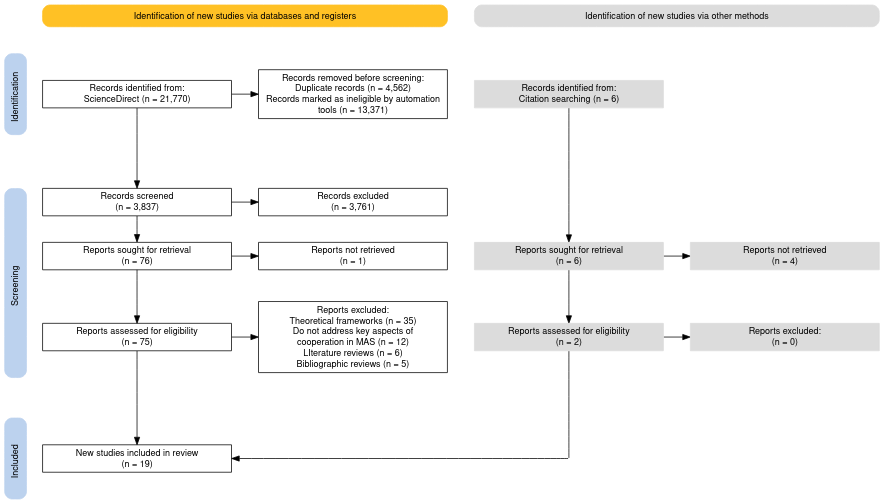
\includegraphics[width=0.8\linewidth]{PRISMA.png}
  \caption{PRISMA Flow Diagram}
  \label{fig:PRISMA}
\end{figure}

\subsubsection{Анализ временного распределения}

Анализ временной шкалы публикаций показывает стабильный, хотя и медленный,
темп появления новых статей в период с 1988 по 2001 год (рис.~\ref{fig:articles-by-year}).
Затем наблюдается десятилетний разрыв до 2011 года,
после которого количество публикаций удвоилось по сравнению с 1988-2001 годами.
Наибольшее число статей (три) было опубликовано в 2021 году
--- последнем году, включённым в данный обзор.
Этот тренд отражает как давнюю историю развития данной научной области,
так и неизменный интерес к ней на протяжении многих лет.

\begin{figure}
  \centering
  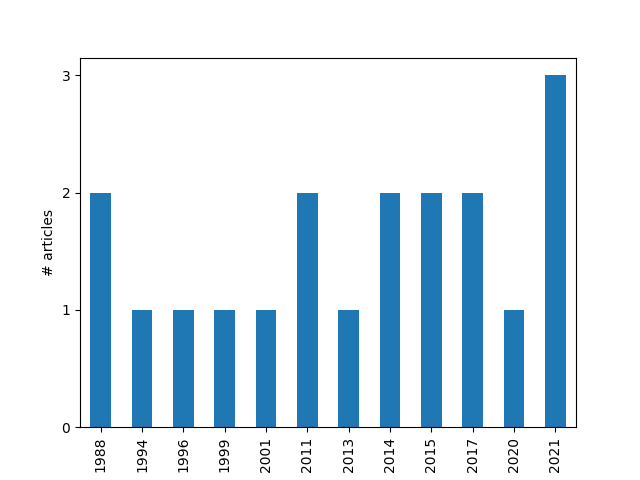
\includegraphics[width=0.8\linewidth]{articles_by_years.png}
  \caption{Статьи по годам}
  \label{fig:articles-by-year}
\end{figure}

\subsubsection{Географическое распределение публикаций}

С учётом совместных исследований лидером в данной области является США,
на долю которых приходится семь публикаций,
что составляет более трети всех рассмотренных работ (рис.~\ref{fig:countries-of-origin}).
На втором месте находится Испания с тремя статьями.
Китай, Австралия, Израиль и Чехия внесли по два исследования каждая.
В то же время Индия, Италия, Португалия, Словакия, Бельгия, Оман, Франция, Тунис, Турция и Нидерланды представлены одной публикацией каждая.

\begin{figure}
  \centering
  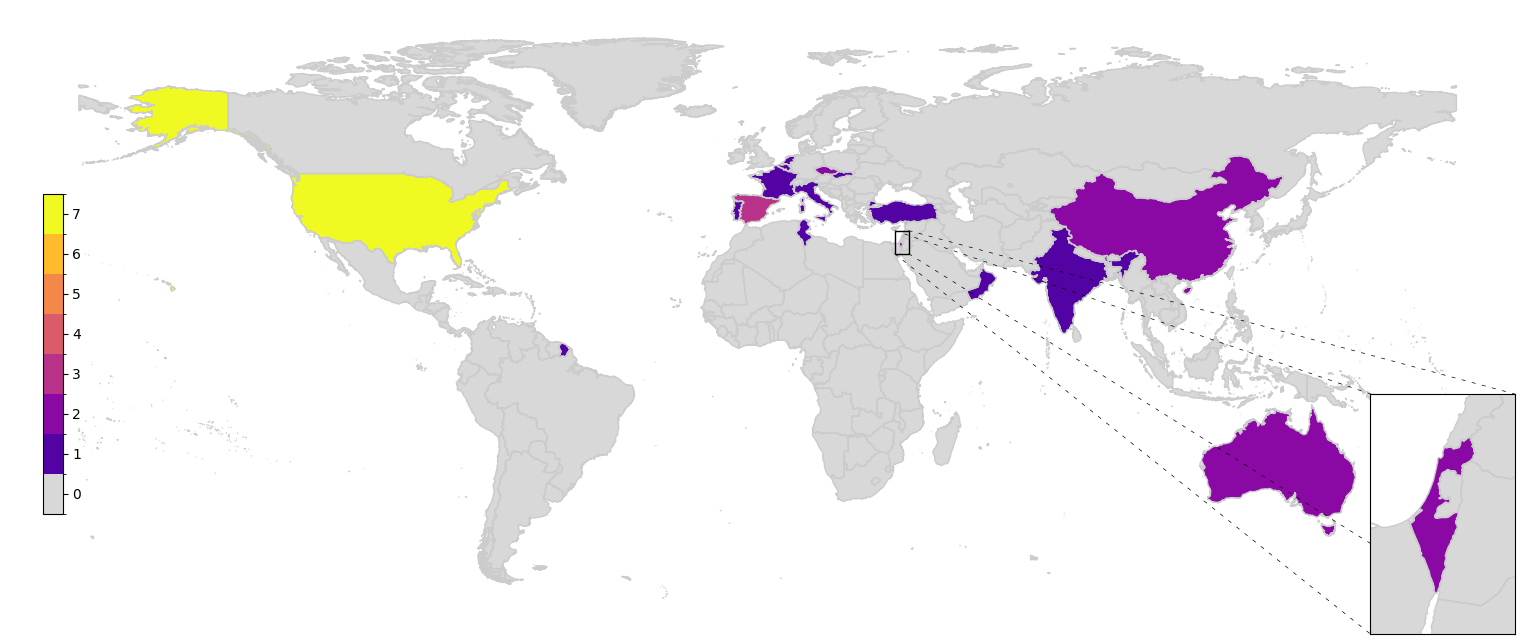
\includegraphics[width=0.8\linewidth]{countries_of_origin.png}
  \caption{Распределение по странам}
  \label{fig:countries-of-origin}
\end{figure}

\subsection{Определение текущих тенденций}

\begin{figure}
  \centering
  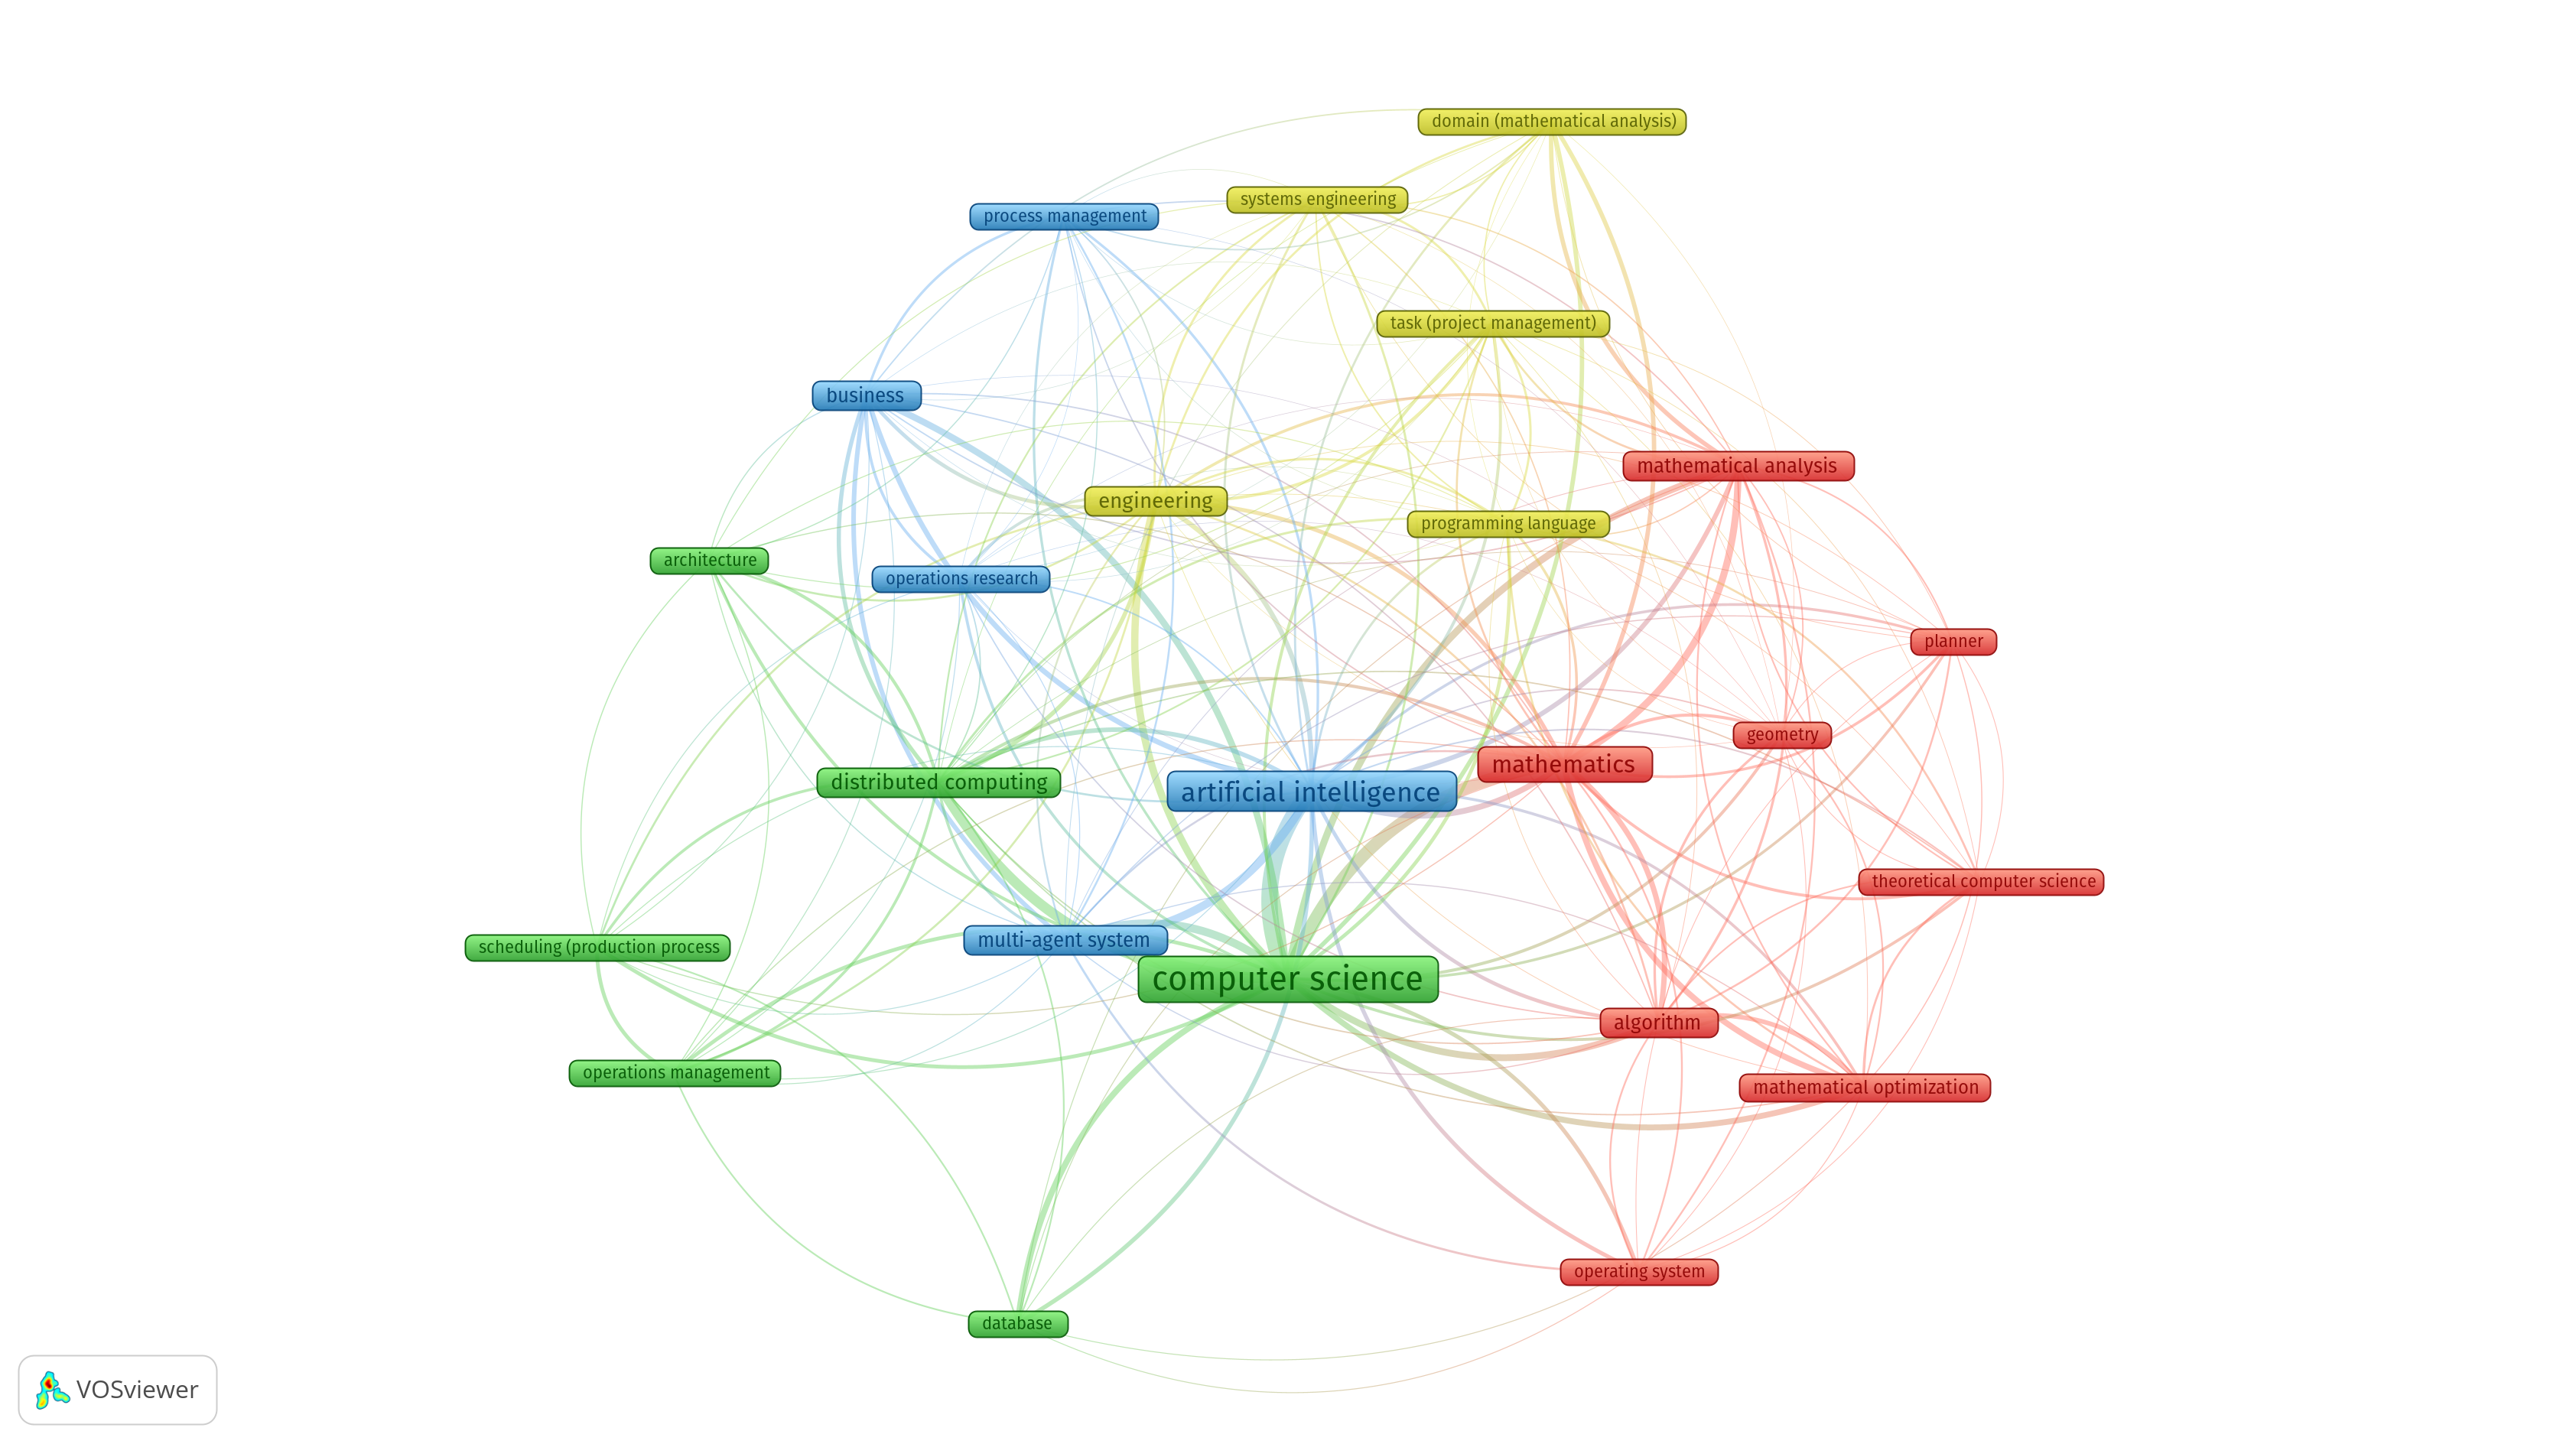
\includegraphics[width=0.8\linewidth]{co-occurence.png}
  \caption{Совместное использование ключевых слов}
  \label{fig:co-occurence}
\end{figure}

Анализируя данные, извлеченные из статей, можно выделить четыре основные области (рис.~\ref{fig:co-occurence}):

\paragraph{Математика}

Этот кластер (красный) акцентирует внимание на математическом моделировании, методах оптимизации и проектировании алгоритмов.
Существуют сильные связи между <<математикой>> и <<математическим анализом>>,
отражающие теоретические основы, а также между <<математикой>> и <<алгоритмом>>, что подчеркивает вычислительные стратегии.

\paragraph{Информатика}

Этот кластер (зеленый) сосредоточен на архитектуре систем, обработке данных и распределенных системах.
Значимые связи включают <<информатику>> с <<распределенными вычислениями>> и <<базой данных>>,
что иллюстрирует вычислительные методы для обработки данных в ресурсоемких задачах.

\paragraph{Искусственный интеллект}

Этот кластер (синий) охватывает интеллектуальные системы, принятие решений и оптимизацию процессов.
Сильные ассоциации наблюдаются между <<искусственным интеллектом>> и <<мультиагентными системами>>,
а также между <<ИИ>> и <<управлением процессами>>.

\paragraph{Инжиниринг и разработка систем}

Этот кластер (желтый) сосредоточен на внедрении и системной инженерии,
противопоставляя себя более теоретическим кластерам, описанным выше.
Существенные связи связывают <<системную инженерию>> с <<управлением задачами>> и <<математический анализ>> с <<управлением задачами>>,
подчеркивая интеграцию аналитических методов в проектирование систем.

Однако самые сильные связи --- между кластерами, особенно между математическими основами и вычислительными системами.
Связи, такие как <<математика>> и <<информатика>>, показывают, что математика является основой информатики,
в то время как <<алгоритм>> и <<искусственный интеллект>> подчеркивают интеграцию алгоритмических подходов в ИИ.
Междисциплинарные связи между <<распределёнными вычислениями>> и <<мультиагентными системами>> подчеркивают распределённые подходы в кооперативном планировании,
а связи между <<инженерией>> и <<искусственным интеллектом>> акцентируют внимание на том,
что, хотя рассматриваемые статьи в основном касаются теоретических приложений,
реальные потребности также находятся в центре внимания этих исследований.
Это не вызывает удивления,
поскольку оно отражает естественный порядок вещей в исследуемой области,
а именно — в области информатики.

\subsection{Синтез результатов}

\subsubsection{Моделирование проблемы}

\paragraph{Представление домена}

Алгоритмические подходы к разрешению конфликтов и кооперативному планированию в MAS
обычно основываются на определении структурированных доменов, в которых взаимодействуют агенты.
Эти домены моделируются с использованием формальных представлений,
таких как графы ограничений~\cite{SHARON201540,SEMIZ2021220},
иерархические сетевые задачи~\cite{FRANKOVIC20017} и архитектуры blackboard~\cite{DURFEE1988268}.
Подобные формализмы способствуют четкому определению целей,
ограничений и взаимозависимостей между агентами~\cite{GROSZ1996269}.
В качестве математических моделей часто используются задачи удовлетворения ограничений,
которые позволяют учитывать требования к принятию решений и накладываемые ограничения~\cite{KOMENDA201476}.
Благодаря этим формализмам агенты могут работать автономно, обеспечивая согласованность с общими целями.

\paragraph{Представление состояний и целей}

Подходы, основанные на моделировании состояний, позволяют агентам отслеживать их прогресс и динамически оценивать изменения в окружающей среде.
Проблемы, как правило, формулируются в виде переходов между состояниями,
где действия определяются для достижения заданных целей~\cite{CHOUHAN2015396}.
Агенты поддерживают локальные представления среды,
дополненные общими ограничениями и возможностями для согласования действий на глобальном уровне~\cite{ROSENSCHEIN1988187}.
Цели могут определяться явно как конечные состояния или неявно через функции полезности,
оценивающие эффективность выполнения задач~\cite{MA2021103823}.
Кроме того, модели часто включают вероятностные методы рассуждения для учета неопределенности,
что повышает устойчивость и надежность принятия решений~\cite{WU2011487}.

\paragraph{Временное и динамическое моделирование}

С учетом динамической природы мультиагентных систем многие подходы интегрируют временные модели
для управления изменяющейся средой~\cite{MA2021103823,LU2014215}.
Для структурирования последовательности задач и координации выполнения
в изменяющихся условиях используются рабочие процессы и событийно-ориентированные фреймворки.
Временные ограничения задают границы временных окон выполнения задач,
обеспечивая синхронизацию между агентами.
Динамические обновления посредством инкрементальных механизмов планирования позволяют адаптироваться в реальном времени,
как это наблюдается в методах с итеративным уточнением и поэтапной корректировкой планов~\cite{SEMIZ2021220}.
Эти методологии позволяют системам реагировать на непредвиденные изменения без необходимости полного перепланирования.

\subsubsection{Стратегии разрешения конфликтов}

\paragraph{Удовлетворение и расслабление ограничений}

Алгоритмы, такие как Conflict-Based Search,
решают конфликты путем итеративного уточнения решений
за счет добавления или ослабления ограничений~\cite{SHARON201540}.
Эти стратегии опираются на пошаговые оценки для эффективного разрешения конфликтов при сохранении оптимальности.
В более динамичных условиях инкрементальные корректировки позволяют системам
устранять неожиданные конфликты в реальном времени без необходимости полного пересмотра планов~\cite{KOMENDA201476}.

\paragraph{Переговоры и торги}

Подходы, основанные на переговорах, используют механизмы распределения задач,
включая модели торгов и аукционов,
для распределения ресурсов и задач между агентами~\cite{GHARRAD2021108282,FRANKOVIC20017,RABELO1994303}.
Эти методы акцентируют кооперативные взаимодействия,
в которых агенты итеративно уточняют соглашения на основе приоритетов и ограничений.
Гибкость в перераспределении задач способствует масштабируемости и способности адаптироваться к изменяющимся условиям.
Динамические корректировки и циклы пересмотра договоренностей обеспечивают устранение возникающих конфликтов в ходе выполнения задач.

\paragraph{Аргументация и мета-рассуждение}

Некоторые фреймворки включают методы аргументации,
позволяя агентам участвовать в структурированных диалогах для разрешения конфликтов~\cite{PAJARESFERRANDO201322,FERRANDO20171}.
Системы аргументации оценивают конкурирующие утверждения,
выявляют несоответствия и приходят к соглашениям через процессы мета-рассуждения.
Этот подход особенно эффективен в сценариях,
требующих объяснительного обоснования решений или согласованных действий в рамках коллективного контекста.
Моделирование обновления убеждений и корректировки предпочтений
в аргументационных механизмах способствует прозрачному принятию решений и адаптивности.

\subsubsection{Механизмы кооперации}

\paragraph{Распределенный и децентрализованный контроль}

Методы распределенного планирования составляют основу кооперативных мультиагентных систем.
Эти подходы избегают централизованного управления~\cite{DURFEE1988268,GRASTIEN2020103271,MA2021103823}
в пользу децентрализованных структур, где агенты действуют независимо,
координируясь через общие коммуникационные протоколы~\cite{ROSENSCHEIN1988187}.
Такая структура повышает масштабируемость, отказоустойчивость и надежность системы,
снижая зависимость от централизованных координаторов.
Протоколы обеспечивают обмен ограничениями и обновлениями, позволяя агентам синхронизировать действия и эффективно использовать ресурсы.

\paragraph{Декомпозиция задач и иерархии}

Методы иерархической декомпозиции задач позволяют разделять сложные проблемы на более мелкие подзадачи,
обеспечивая их параллельное выполнение и улучшенный контроль~\cite{JUNG1999149}.
Эти подходы используют многоуровневые структуры планирования,
где высокоуровневые цели определяют низкоуровневые действия.
Иерархии способствуют разрешению конфликтов за счет изоляции зависимостей внутри групп задач,
что упрощает управление взаимодействиями агентов.
Такая структура также поддерживает масштабируемость и модульное планирование~\cite{RODRIGUEZ201113005},
делая ее подходящей для крупных систем.

\paragraph{Динамические обновления и адаптация}

Механизмы динамической адаптации обеспечивают способность мультиагентных систем реагировать на изменения в окружающей среде.
Циклы обратной связи и методы итеративного обучения позволяют агентам непрерывно оценивать производительность
и корректировать планы на основе наблюдаемых результатов~\cite{LU2014215}.
Методы восстановления планов и инкрементальной корректировки повышают устойчивость системы,
сводя к минимуму сбои в ходе выполнения задач.
Эти механизмы особенно важны в динамичных доменах, где условия изменяются непредсказуемо.

\subsubsection{Оценка эффективности}

Оценка эффективности представленных методологий выявляет их сильные и слабые стороны.
Методы удовлетворения ограничений отличаются математической строгостью и масштабируемостью,
что делает их эффективными в структурированных доменах,
где ограничения могут быть четко заданы~\cite{STOLBA2017175}.
Однако в условиях высокой динамичности или неопределенности они могут требовать дополнительных адаптивных слоев~\cite{SHARON201540}.
Переговорные подходы демонстрируют гибкость и адаптивность за счет динамического распределения задач.
Итеративная корректировка и пересмотр соглашений делают их пригодными для открытых и изменяющихся сред.
Тем не менее, их зависимость от коммуникационных протоколов может вызывать накладные расходы в условиях ограниченной пропускной способности или задержек~\cite{PAJARESFERRANDO201322}.
Аргументационные фреймворки эффективны в областях, требующих обоснования решений,
обеспечивая прозрачность и доверие в коллективном принятии решений.
Однако их вычислительная сложность может быть ограничивающим фактором в масштабных системах с многочисленными агентами~\cite{FERRANDO20171}.
Кооперативные механизмы, основанные на распределенном управлении и иерархической декомпозиции,
демонстрируют высокую масштабируемость и отказоустойчивость,
что делает их эффективными в больших децентрализованных системах~\cite{MA2021103823}.
Однако они могут требовать сложных протоколов координации для обеспечения согласованности, особенно в системах с разнородными агентами~\cite{JUNG1999149}.
Методы динамической адаптации повышают устойчивость и оперативность,
делая их незаменимыми в условиях неопределенности и изменений~\cite{LU2014215}.
Однако их эффективность часто зависит от качества механизмов обратной связи
и способности балансировать исследование новых решений и использование имеющегося опыта.

\section{Обсуждение}

\subsection{Обобщение данных}

Этот обзор рассматривает стратегии разрешения конфликтов и механизмы кооперации в мультиагентных системах,
фокусируясь на моделировании, методах решения и взаимодействии.
Формальные представления, такие как задачи удовлетворения ограничений,
иерархические сети задач и временные модели, служат структурной основой~\cite{GROSZ1996269,KOMENDA201476}.
Эти методы учитывают ограничения и неопределенности, поддерживая координацию через основанное на состояниях рассуждение и обновления~\cite{STOLBA2017175,LU2014215}.

Разрешение конфликтов опирается на удовлетворение ограничений, переговоры и аргументационные структуры.
Конфликтно-ориентированный поиск уточняет решения для динамических сред~\cite{SHARON201540}.
Переговоры и торговля улучшают распределение ресурсов,
но увеличивают коммуникационные издержки~\cite{PAJARESFERRANDO201322,FRANKOVIC20017}.
Аргументационные методы повышают прозрачность, но страдают от проблем масштабируемости~\cite{FERRANDO20171}.

Кооперация достигается через распределенное управление и иерархии задач,
обеспечивая масштабируемость и отказоустойчивость~\cite{MA2021103823,JUNG1999149}.
Динамическая адаптация повышает устойчивость с помощью итеративного обучения и обратной связи~\cite{SEMIZ2021220}.

Эффективность методов зависит от условий: модели ограничений успешны в структурированных средах,
переговоры гибки в динамических сценариях, аргументация повышает объяснимость решений.
Однако остаются вызовы масштабируемости, адаптивности и вычислительных затрат,
требующие усовершенствованных критериев оценки и универсальных методологических основ.
Дальнейшие исследования должны устранить эти ограничения для создания надежных и масштабируемых решений.

\subsection{Ограничения}

Можно выделить несколько потенциальных ограничений.  

\subsubsection{Отсутствие унифицированных стандартов оценки}

Отсутствие единых кросс-доменных критериев оценки в различных исследованиях
создает проблему для проведения содержательных сравнений.
Например, одни работы делают акцент на вычислительной эффективности,
тогда как другие отдают приоритет адаптивности или стабильности.

\subsubsection{Зависимость от данных, полученных на основе симуляций}

Значительная часть представленных в рассмотренных исследованиях данных получена из симуляций,
а не из реальных внедрений. Хотя симуляции обеспечивают контролируемые условия тестирования,
они могут не полностью отражать сложности развертывания мультиагентных систем в динамических реальных средах.  

Устранение этих ограничений в будущих исследованиях за счет расширения критериев включения,
стандартизации метрик и интеграции реальных кейс-стадий позволит повысить полноту и актуальность обзора.

\section{Заключение}

Этот обзор охватывает систематический анализ методологий и структур,
используемых для разрешения конфликтов и кооперативного планирования в мультиагентных системах.
Результаты подчеркивают сильные и слабые стороны современных подходов,
включая задачи удовлетворения ограничений, модели переговоров и децентрализованные структуры.
Хотя эти методы демонстрируют масштабируемость, адаптивность и вычислительную эффективность,
остаются пробелы в оценочных метриках и практическом применении.  

Данное исследование подчеркивает необходимость стандартизированных тестов и показателей производительности
для обеспечения сопоставимости различных подходов.
Кроме того, будущие исследования должны сосредоточиться на интеграции динамической адаптивности и реальных внедрений,
чтобы решать возникающие вызовы в средах мультиагентных систем.
Повышение масштабируемости и устойчивости за счет гибридных методологий и передовых методов обучения
будет ключевым фактором дальнейшего развития приложений MAS.  

\vspace{\baselineskip}

\begin{authorcontributions}
  Концептуализация, написание --- подготовка первоначального варианта: Григорий Васильевич Матюхин;
  руководство, написание --- рецензирование и редактирование: Андрей Николаевич Виноградов.
  Все авторы прочитали и согласились с опубликованной версией рукописи.
\end{authorcontributions}

\begin{funding}
  Данное исследование не получало внешнего финансирования.
\end{funding}

\begin{dataavailability}
  В ходе исследования были проанализированны данные из 19 статей,
  посвященных разрешению конфликтов в мультиагентных системах. 
  С промежуточными результатами можно ознакомится по ссылке \url{https://gmatiukhin.site/articles/MAS-Conflict-Solving-Review/}
\end{dataavailability}

\begin{conflictsofinterest}
  Авторы заявляют об отсутствии конфликта интересов.
\end{conflictsofinterest}

%%
%% Define the bibliography file to be used
\printbibliography

%%
%% If your work has an appendix, this is the place to put it.
% \appendix
%
% \section{Онлайн-ресурсы}
%
% \begin{itemize}
% \item Overleaf: \url{https://www.overleaf.com/read/vjvjpsqrqjhj#86e97e}.
% \item Overleaf (russian): \url{https://www.overleaf.com/read/yjmkpnvgqzdk#bf8ccf}.
% \end{itemize}

\end{document}

%%% Local Variables:
%%% mode: LaTeX
%%% TeX-master: t
%%% End:
